% \documentclass[12pt]{article}
\documentclass[12pt,fleqn]{article}
\usepackage[utf8]{inputenc}
\usepackage[russian]{babel}
\usepackage{graphicx}
\usepackage{array}
\usepackage[a4paper, left=1cm, right=1cm, top=1.27cm, bottom=1.27cm]{geometry}
\usepackage{setspace}
\usepackage{tabularx}
\usepackage{makecell}
\usepackage{longtable}
\usepackage{multirow}
\usepackage{caption}
\usepackage{amsmath}
\usepackage{amssymb}
\usepackage{ragged2e}
\onehalfspacing


\begin{document}


\begin{table}[h]
    \centering
    \renewcommand{\arraystretch}{1.5}
    \begin{tabular}{m{11cm}m{6cm}}
        \begin{center}
            \textbf{Университет ИТМО}\\
            \textbf{Физико-технический мегафакультет}\\
            \textbf{Физический факультет}
        \end{center} 
        & 
        \begin{center}
            
\includegraphics[height=1.3cm]{logo.jpg}
        \end{center} \\
    \end{tabular}
\end{table}

\noindent\makebox[\linewidth]{\rule{\textwidth}{2pt}}

\vspace{10pt}

\begin{table}[h]
    \centering
    \renewcommand{\arraystretch}{1.7}
    \begin{tabular}{p{4cm}p{4cm}p{8cm}}
        Группа N3250 & & К работе допущен \underline{\hspace{4cm}} \\
        Студенты & \hfill \multirow[0pt]{3}{*}{\makecell[c]{Пахомов В.Ю \\ Булин М.М \\ Рулев М.Ю}}  & Работа выполнена \underline{\hspace{4cm}} \\
        & & \\
        & & \\
        \multicolumn{2}{l}{Преподаватель Рудель А.Е}  & Отчет принят \underline{\hspace{5cm}} \\
    \end{tabular}
\end{table}

\begin{center}
    \fontsize{20pt}{21.5pt} \selectfont
    \textbf{Рабочий протокол и отчет по} \\
    \textbf{лабораторной работе № 3.06}
\end{center}

\noindent\makebox[\linewidth]{\rule{\textwidth}{1pt}}
\noindent\makebox[\linewidth]{\rule{\textwidth}{1pt}}

\begin{justify}
    \textbf{1. Цель работы}
    \begin{enumerate}
        \item Определение значений электрического смещения насыщения $D_S$, остаточной поляризации $P_r$, коэрцитивной силы $E_C$ для предельной петли гистерезиса сегнетоэлектрика.
        \item Расчет диэлектрических потерь за цикл переполяризации сегнетоэлектрика. 
        \item Получение зависимостей смещения $D$ и диэлектрической проницаемости $\varepsilon$ от напряженности электрического поля $E$.
        \item Определение значений начальной и максимальной диэлектрической проницаемости.
    \end{enumerate}
\end{justify}

\begin{justify}
    \textbf{2. Задачи, решаемые при выполнении работы} \\
    Нахождение электрического насыщения, остаточночной поляризации, коэрцитивной силы, рассчет диэлектрических потерь за цикл переполяризации, определение начальной и максимальной проницаемости.
\end{justify}

\begin{justify}
    \textbf{3. Объект исследования} \\
    Объектом исследования является Сегнетоэлектрический конденсатор (вариконд) типа ВК2-4, установленный на стенде С3-РМ02.
\end{justify}

\begin{justify}
    \textbf{4. Метод экспериментального исследования} \\
    Метод осциллографирования петли гистерезиса на экране измерительного прибора ИСХ1, когда напряжение, пропорциональное напряженности поля $E$, подается на вход горизонтального отклонения, а напряжение, пропорциональное электрическому смещению $D$, на вход вертикального отклонения. 
\end{justify}

\begin{justify}
    \textbf{5. Рабочие формулы и исходные данные} \\
    $R_1 = 47 \text{кОМ} \pm 10\%$ \\
    $R_2 = 470 \text{кОМ} \pm 10 \% $ \\
    $C_1 = 1 \text{мкФ} \pm 10 \% $ \\
    $C_2 = 0.01 \text{мкФ} \pm 10 \% $ \\
    Площадь пластин конденсатора: $ 500 \text{мм}^2 \pm 10 \% $ \\
    Толщина сегнетоэлектрика: $0.5 \text{мм} \pm 10 \% $ \\
    $D_S = 3.1 \quad D_r = 1.3$ \\
    $E_s = 2.7 \quad E_c = 0.7$
    \[ D = \sigma = \frac{q}{S} = \frac{C_2U_{C_2}}{S} = \frac{C_1}{S} \cdot U_{C_1} \]
    \[ E = \frac{U_{C_2}}{d} = \frac{U}{d} = \frac{R_1 + R_2}{R_1} \cdot \frac{U_{R_1}}{d} \]
    \[ \tg \delta = \frac{1}{\pi} \cdot \frac{\oint DdE}{D_sE_s} \]
\end{justify}


\begin{flushleft}
    \textbf{6. Измерительные приборы} \\
    \begin{table}[h]
    \centering
    \renewcommand{\arraystretch}{1.5}
    \begin{tabular}{|c|c|c|c|c|}
        \hline
        № п/п & Наименование & Тип прибора & Используемый диапазон & Погрешность прибора\\
        \hline
        1 & С3-РМ02 & Стенд & - & - \\
        \hline
        2 & ИСХ-1 & Лабораторный & - & - \\
        \hline
    \end{tabular}
    \end{table}
\end{flushleft}


\begin{flushleft}
    \textbf{7. Схема установки} \\
    \begin{figure}[h!]
        \centering
        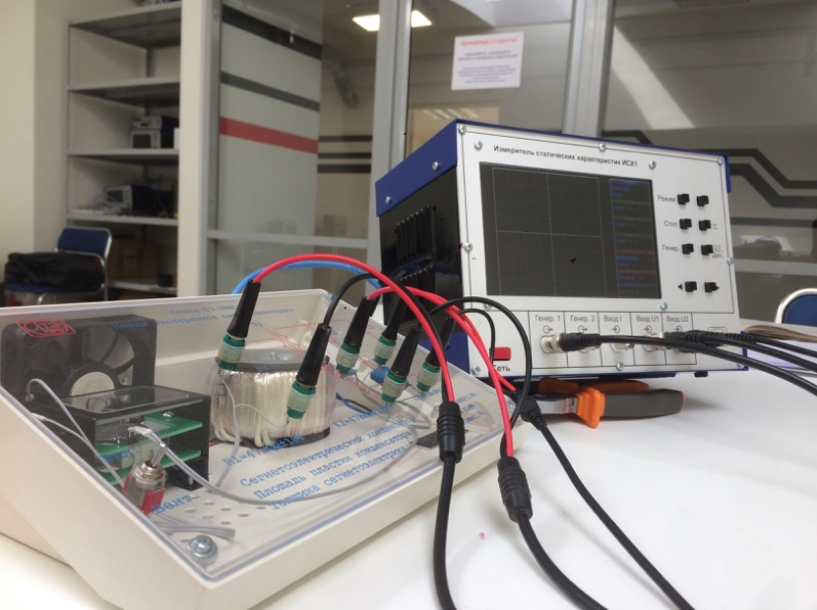
\includegraphics[height=10cm]{schema2.png}
        \caption{Общий вид лабораторной установки}
    \end{figure}
    \begin{figure}[h!]
        \centering
        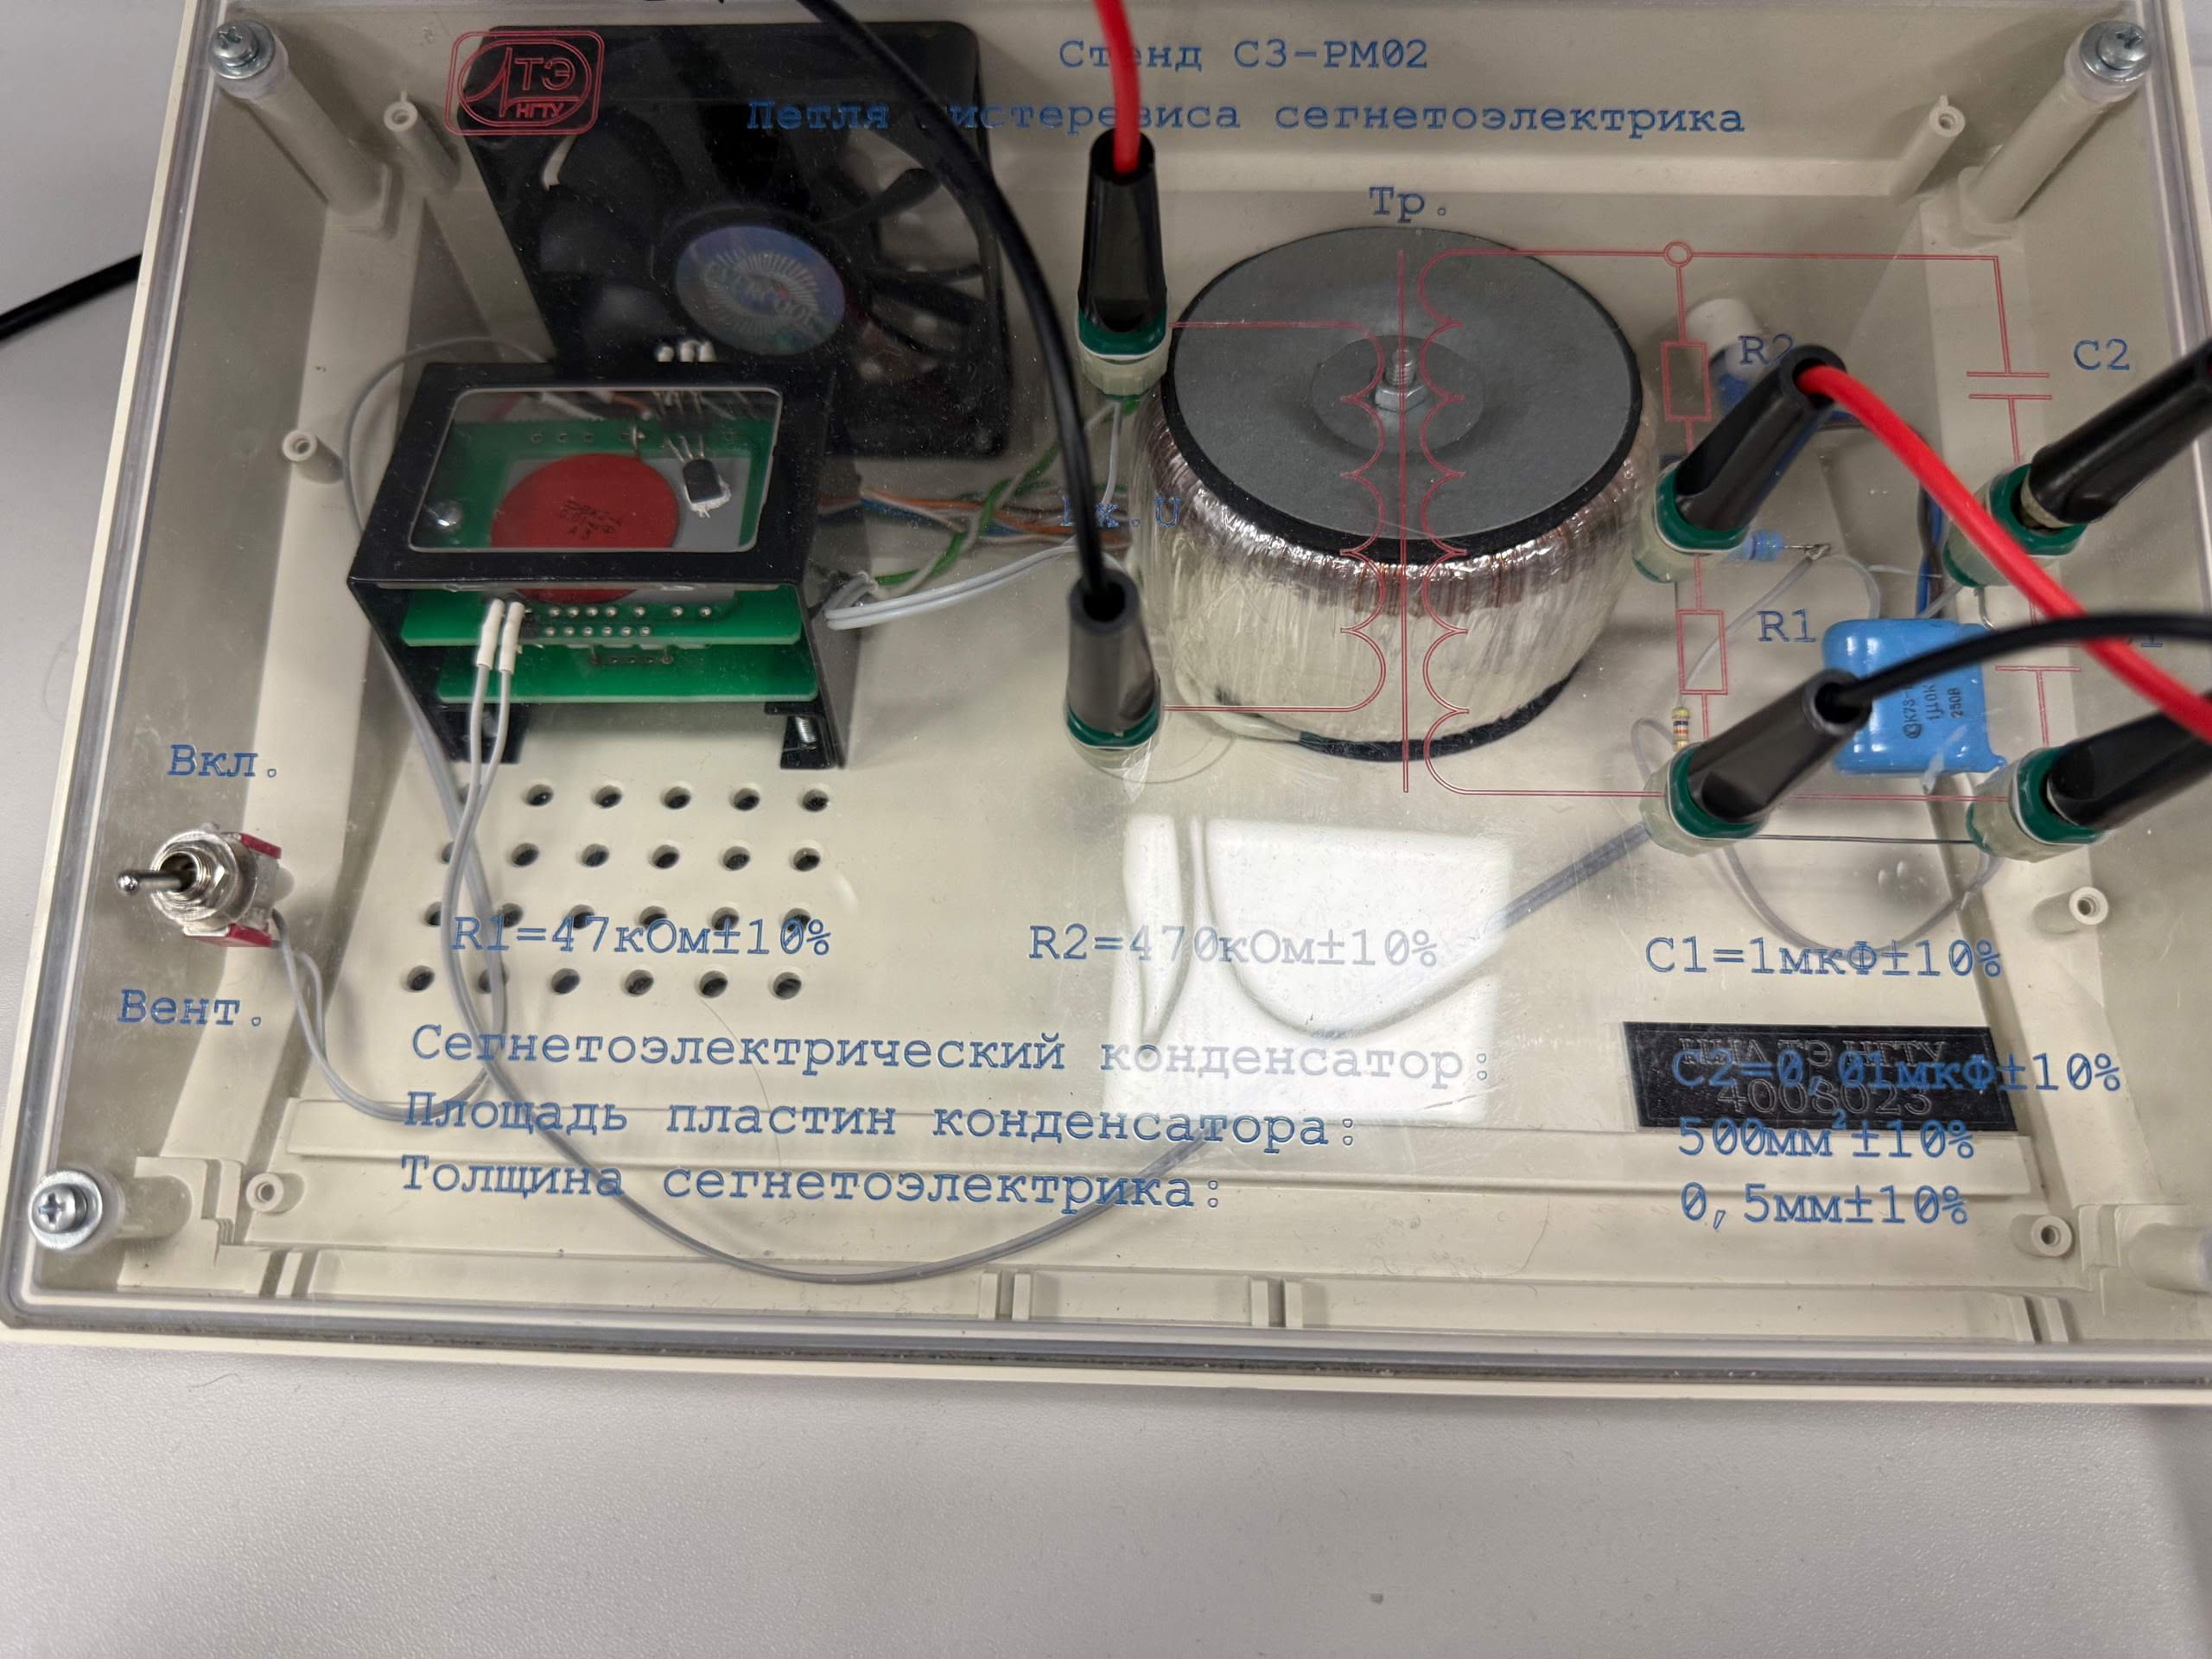
\includegraphics[height=8cm]{schema1.jpg}
        \caption{Внешний вид стенда С3-РМ02}
    \end{figure}
    
\end{flushleft}


\newpage


\begin{flushleft}
    \textbf{8. Результаты прямых измерений и их обработки} \\

    \begin{table}[h!]
    \centering
    \caption{Зависимость диэлектрической проницаемости сегнетоэлектрика от напряженности электрического поля}
    \begin{tabular}{|c|c|c|c|c|c|c|c|c|}
    \hline
    № & $U, \, \text{B}$ & $K_x, \, \text{B/дел}$ & $K_y, \, \text{B/дел}$ & $X, \, \text{дел}$ & $Y, \, \text{дел}$ & $E, \, \text{B/м}$ & $D, \, \text{Кл/м}^2$ & $\varepsilon$ \\
    \hline
    1 & 17 & 5 & 5 & 2.7 & 3.1 & 297 000 & 0,0310 & 11 794 \\
    \hline
    2 & 15 & 5 & 5 & 2.3 & 3 & 253 000 & 0,0300 & 13 398 \\
    \hline
    3 & 13 & 5 & 5 & 2.1 & 2.7 & 231 000 & 0,0270 & 13 207 \\
    \hline
    4 & 11 & 5 & 5 & 1.6 & 2.2 & 176 000 & 0,0220 & 14 124 \\
    \hline
    5 & 9 & 2 & 5 & 3.5 & 1.6 & 154 000 & 0,0160 & 11 740 \\
    \hline
    6 & 7 & 2 & 2 & 2.7 & 2.7 & 118 800 & 0,0108 & 10 272 \\
    \hline
    7 & 5 & 2 & 2 & 2 & 1.6 & 88 000 & 0,0064 & 8 217 \\
    \hline
    8 & 4.4 & 1 & 1 & 3.5 & 2.5 & 77 000 & 0,0050 & 7 337 \\
    \hline
    9 & 3.8 & 1 & 1 & 3 & 1.8 & 66 000 & 0,0036 & 6 163 \\
    \hline
    10 & 3.2 & 1 & 1 & 2.5 & 1.3 & 55 000 & 0,0026 & 5 341 \\
    \hline
    11 & 2.6 & 1 & 0.5 & 2 & 1.6 & 44 000 & 0,0016 & 4 109 \\
    \hline
    12 & 2 & 0.5 & 0.5 & 3.1 & 1.1 & 34 100 & 0,0011 & 3 645 \\
    \hline
    13 & 1.4 & 0.5 & 0.1 & 2.1 & 3.2 & 23 100 & 0,00064 & 3 131 \\
    \hline
    14 & 0.8 & 0.2 & 0.05 & 3 & 3 & 13 200 & 0,00030 & 2 568 \\
    \hline
    15 & 0.2 & 0.05 & 0.02 & 2.9 & 1.6 & 3 190 & 0,000064 & 2 267 \\
    \hline
    \end{tabular}
    \end{table}
    Пример расчетов для первой строки таблицы:
    \[ E = \frac{R_1 + R_2}{R_1} \cdot \frac{U_{R_1}}{d} = \frac{R_1 + R_2}{R_1} \cdot \frac{X K_x}{d} = \frac{470 + 47}{47} \cdot \frac{2.7 \cdot 5}{0.5 \cdot 10^{-4}} = 297000 \, \text{В}/\text{м} \]
    \[ D = \frac{C_1}{S} \cdot U_{C_1} = \frac{C_1}{S} \cdot Y \cdot K_y = \frac{10^{-6}}{5 \cdot 10^{-4}} \cdot 3.1 \cdot 5 = 0.0310 \, \text{Кл}/\text{м}^2 \]
    \[ \varepsilon = \frac{D}{\varepsilon_0 E} = \frac{0.0310}{8.85 \cdot 10^{-12} \cdot 297000} = 11 794 \] 
   
\end{flushleft}


\newpage


\begin{justify}
    \textbf{9. Расчет результатов косвенных измерений (таблицы, примеры расчетов)} \\
    Значение коэрцитивного поля:
    \[ E_c = \frac{R_1 = R_2}{R_1} \cdot \frac{E_{c,\text{дел}} \cdot K_x}{d} = \frac{470 + 47}{47} \cdot \frac{0.7 \cdot 5}{0.5 \cdot 10^{-4}} = 77000 \pm 18\% \; \text{В}/\text{м} \]
    Электрическая индукция в состоянии насыщения:
    \[ D = \frac{C_1}{S} \cdot D_{s,\text{дел}} \cdot K_y = \frac{10^{-6}}{5 \cdot 10^{-4}} \cdot 3.1 \cdot 5 = 0.031 \pm 14\% \; \text{Кл}/\text{м}^2 \]
    Остаточная поляризация:
    \[ D \approx P \; \Rightarrow \; P_r = \frac{C_1}{S} \cdot D_{r,\text{дел}} \cdot K_y = \frac{10^{-6}}{5 \cdot 10^{-4}} \cdot 1.3 \cdot 5 = 0.013 \pm 16\% \; \text{Кл}/\text{м}^2 \]

    Площадь петли гистеризиса примерно 8 $\text{дел}^2$
    \[ \tg \delta = \frac{1}{\pi} \cdot \frac{\oint DdE}{D_sE_s} = \frac{1}{\pi} \cdot \frac{S}{D_sE_s} = \frac{1}{3.14} \cdot \frac{8}{3.1 \cdot 2.7} \approx 0.304 \]
    Энергия потерь в единице объема:
    \[ w_r = \oint DdE = S_{\text{дел}} \cdot C_E \cdot C_D = 8 \cdot 5 \cdot 22000 \cdot 5 \cdot 0.002 = 8800 \; \text{Дж}/\text{м}^3 \]
\end{justify}

\begin{justify}
    \textbf{10. Расчет погрешностей измерений (для прямых и косвенных измерений)} \\
    \[ \frac{\Delta E}{E} \approx \sqrt{\delta R^2 + \delta d^2 + \Big( \frac{\Delta E_{\text{дел}}}{E_{\text{дел}}}\Big)^2} \approx \sqrt{0.1^2 + 0.1^2 + (0.1/0.7)^2} \approx 18 \% \]
    \[ E_c = 77000 \pm 14000 \; \text{В}/\text{м} \]
    \[ \frac{\Delta D}{D} \approx \sqrt{\delta C^2 + \delta S^2 + \Big( \frac{\Delta D_{\text{дел}}}{D_{\text{дел}}}\Big)^2} \approx \sqrt{0.1^2 + 0.1^2 + (0.1/3.1)^2} \approx 14 \% \]
    \[ D_s = 0.031 \pm 0.004 \; \text{Кл}/\text{м}^2 \]
    \[ \frac{\Delta P}{P} \approx \sqrt{\delta C^2 + \delta S^2 + \Big( \frac{\Delta D_{\text{дел}}}{D_{\text{дел}}}\Big)^2} \approx \sqrt{0.1^2 + 0.1^2 + (0.1/1.3)^2} \approx 16 \% \]
    \[ P_r = 0.013 \pm 0.002 \; \text{Кл}/\text{м}^2 \]
    \[ \delta_{\varepsilon} = \sqrt{\delta_D^2 + \delta_E^2} = \sqrt{0.14^2 + 0.18^2} = \sqrt{0.0196 + 0.0324} = \sqrt{0.052} \approx 0.228 \; (\approx 23\%) \]
\end{justify}


\newpage


\begin{justify}
    \textbf{11. Графики (перечень графиков, которые составляют Приложение 2)} \\
    \begin{figure}[h!]
        \centering
        
\includegraphics[height=10cm]{graphic1.png} \\
        \caption{График зависимости $D = D(E)$}
    \end{figure}
    
    \begin{figure}[h!]
    \centering
    
\includegraphics[height=10cm]{graphic2.png} \\
    \caption{График зависимости $\varepsilon = \varepsilon(E)$}
    \end{figure}
\end{justify}


\newpage


\begin{justify}
    \textbf{12. Окончательные результаты} \\
    \[ E_c = 77000 \pm 14000 \text{ В/м} \]
    \[ \Delta E_c \approx 18\% \]
    \[ D_s = 0.031 \pm 0.004 \text{ Кл/м}^2 \]
    \[ \Delta D_s \approx 14\% \]
    \[ P_r = 0.013 \pm 0.002 \text{ Кл/м}^2 \]
    \[ \Delta P_r \approx 16\% \]
    \[ \varepsilon_{\text{макс}} \approx 14124 \]
    \[ \varepsilon_{\text{нач}} \approx 2267 \]
    \[ w_r = 8800 \text{ Дж/м}^3 \]
    \[ S_{\text{петли}} \approx 8 \text{ дел}^2 \]
    \[ \delta_{\varepsilon} \approx 23\% \]
\end{justify}

\begin{justify}
    \textbf{13. Выводы и анализ результатов работы} \\
    
    Проведённая лабораторная работа позволила изучить ключевые электрические свойства сегнетоэлектриков. В ходе работы была снята предельная петля гистерезиса, анализ которой подтвердил наличие остаточной поляризации и коэрцитивной силы. Были определены численные значения основных параметров: электрическое смещение насыщения составило $D_s = (0.031 \pm 0.004)$ Кл/м$^2$, коэрцитивная сила $E_c = (77 \pm 14)$ кВ/м, а остаточная поляризация $P_r = (0.013 \pm 0.002)$ Кл/м$^2$. Эти результаты демонстрируют способность сегнетоэлектрика сохранять поляризацию после снятия внешнего поля и требуют значительного обратного поля для снятия остаточной поляризации.

    Исследование зависимости диэлектрической проницаемости от напряженности электрического поля выявило её нелинейность. Диэлектрическая проницаемость резко возрастает в слабых полях, достигая максимального значения ($\varepsilon_{\max} \approx 14124$) при $E = 176$ кВ/м, а затем уменьшается, что типично для сегнетоэлектриков в области насыщения. Была определена начальная диэлектрическая проницаемость $\varepsilon_{\text{init}} \approx 2267$. Расчет тангенса угла диэлектрических потерь ($\text{tg}\delta \approx 0.304$), проведённый через площадь петли гистерезиса, продемонстрировал существенные потери энергии на переполяризацию ($w_r = 8800$ Дж/м$^3$), что является следствием процессов переориентации доменов.

    Таким образом, работа подтвердила фундаментальные свойства сегнетоэлектриков --- нелинейность характеристик, гистерезис и высокие диэлектрические потери.
\end{justify}

\begin{justify}
    \textbf{14. Дополнительные задания}
\end{justify}

\begin{justify}
    \textbf{15. Выполнение дополнительных заданий}
\end{justify}

\begin{justify}
    \textbf{16. Замечания преподавателя (исправления, вызванные замечаниями преподавателя, также помещают в этот пункт)}
\end{justify}

\end{document}
